\section{Theorie}

Der Operationsverstärker ist eine integrierte Schaltung, die aus mehreren Transistoren zusammengesetzt ist.
Der Name ergibt sich daraus, dass mit einem Operationsverstärker durch geschickte Beschaltung eine Vielzahl mathematischer Operationen realisiert werden können.

Die Ausgangsspannung ist die Differenz der Eingangsspannungen, die verstärkt und auf die Betriebsspannungen begrenzt ist.

\subsection{Der ideale Operationsverstärker}

\begin{figure}
	\centering
	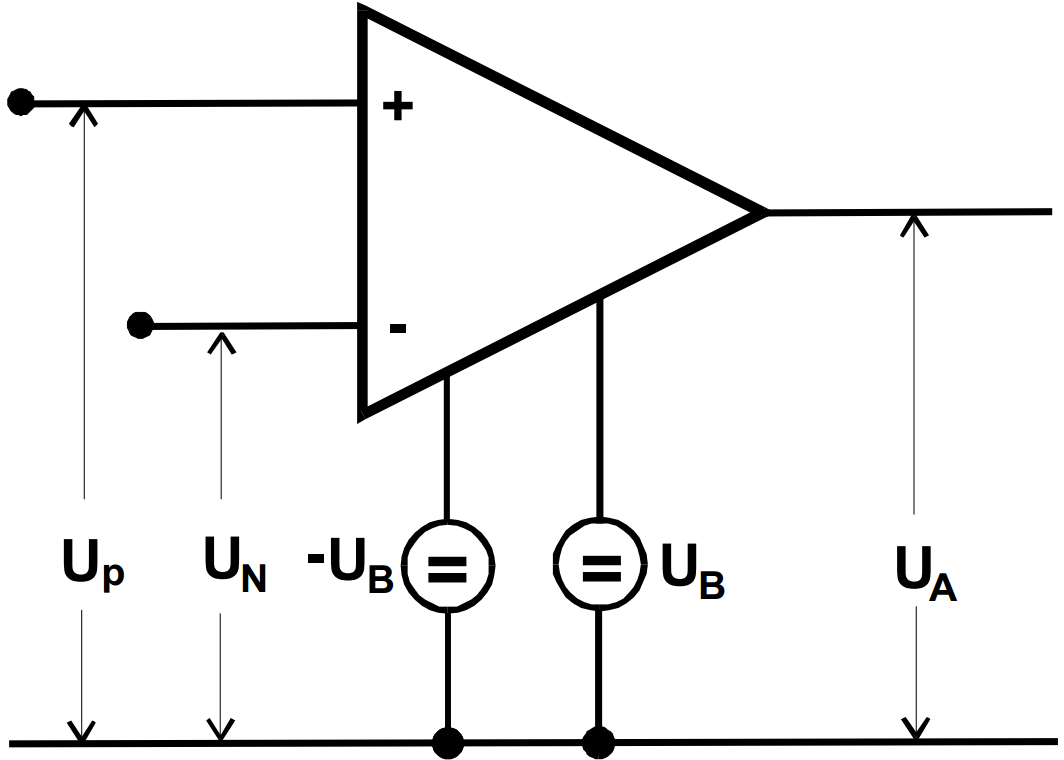
\includegraphics[width=0.6\textwidth]{img/op.png}
	\caption{Schaltsymbol des Operationsverstärkers \cite{v51}}
	\label{fig:op}
\end{figure}

Das Schaltbild eines Operationsverstärkers is in Abbildung \ref{fig:op} dargestellt.
Der OP hat zwei Eingänge, an denen die Spannungen $U_p$ und $U_N$ anliegen.
Die Spannung am Ausgang heißt $U_A$.
An zwei weiteren Eingängen wird die positive und negative Betriebsspannung $U_B$ angelegt.

Die Ausgangsspannung ist die verstärkte Differenz der Eingangsspannungen, also
\begin{align}
	U_A = V \left(U_p - U_N\right).
\end{align}
Dabei ist $V$ die Leerlaufverstärkung.
Eine Erhöhung von $U_n$ führt zu einer Verringerung der Ausgangsspannung.
Deswegen wird der Eingang von $U_n$ invertierender Eingang genannt.
Der andere Eingang heißt entsprechend nicht-invertierender Eingang.

Die Ausgangsspannung ist auf die Höhe der Betriebsspannung begrenzt, das heißt:
\begin{align}
	-U_B < U_A < U_B
\end{align}

Daraus ergibt sich die Kennlinie des Operationsverstärkers, die in Abbildung \ref{fig:kennlinie} dargestellt ist.
\begin{figure}
	\centering
	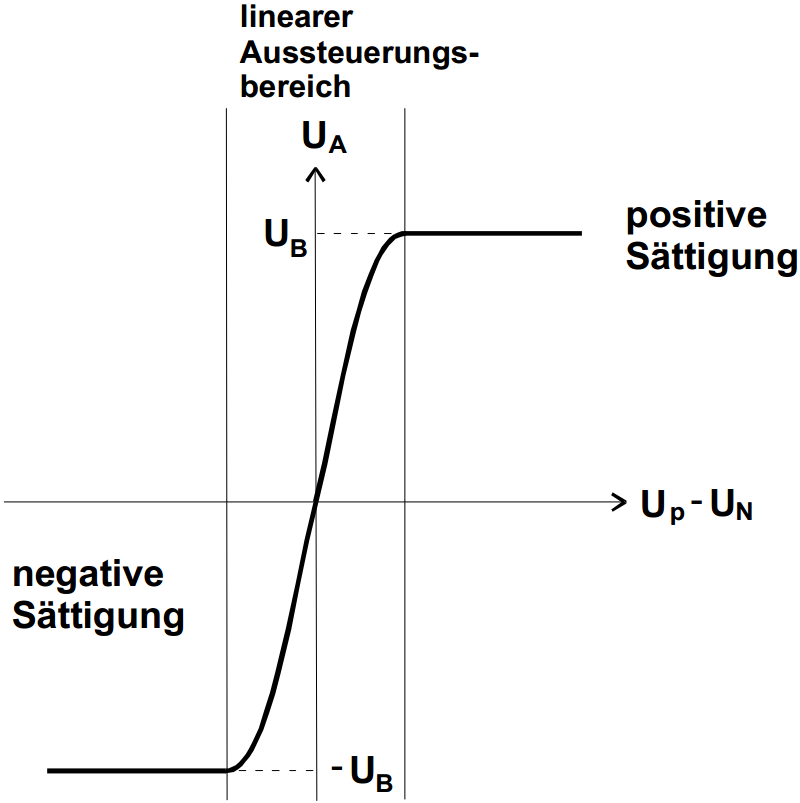
\includegraphics[width=0.5\textwidth]{img/kennlinie.png}
	\caption{Kennlinie des Operationsverstärkers \cite{v51}}
	\label{fig:kennlinie}
\end{figure}

Beim idealen Bauteil ist $V \rightarrow \infty$.
Folglich nimmt die Ausgangsspannung immer $\pm U_B$ an und der OP arbeitet als Komparator.
Weiterhin fließt beim idealen Bauteil kein Strom in die Eingänge.
Dies entspricht einem unendlich großen Eingangswiderstand $r_e$.
Der Ausgang hingegen kann einen beliebig großen Strom liefern, entsprechend eines Ausgangswiderstands $r_a$ von $0$.

\subsection{Der reale Operationsverstärker}

Beim realen Operationsverstärker nehmen die Leerlaufverstärkung, die Eingangswiderstände und der Ausgangswiderstand endliche Werte an.
Es gibt einige weitere Effekte, die im Folgenden beschrieben werden.

\subsubsection{Gleichtaktverstärkung}
Die Gleichtaktverstärkung ist die Spannung, die am Ausgang gemessen wird, wenn an beiden Eingängen die gleiche Spannung $U_{Gl}$ angelegt wird.
Sie ist idealerweise $0$.
\begin{align}
	V_{Gl} = \frac{\Delta U_A}{\Delta U_{Gl}}
\end{align}

\subsubsection{Eingangswiderstand}

Da die Eingangswiderstände nicht unendlich sind, fließen in die Eingänge die Ströme $I_p$ und $I_N$.
Der Differenzeingangswiderstand wird definiert als
\begin{align}
	r_D =
	\begin{cases}
		\frac{\Delta U_p}{\Delta I_p} \quad & \text{für} \quad U_n = 0\\
		\frac{\Delta U_N}{\Delta I_N} \quad & \text{für} \quad U_p = 0
	\end{cases}
\end{align}
und der Gleichtakteingangswiderstand als 
\begin{align}
	r_{Gl} = \frac{\Delta U_{Gl}}{\Delta I_{Gl}},
\end{align}
mit $Up = U_N = U_{Gl}$ und $I_{Gl} = I_p + I_N$.

\subsubsection{Offsetspannung}
Legt man am realen OP an beiden Eingängen die Spannung $0$ an, ist die Ausgangsspannung nicht wie erwartet $0$.
Die Offsetspannung ist definiert als die Differenz der Eingangsspannungen wenn die Ausgangsspannung $0$ ist.
\begin{align}
	U_0 = U_p - U_N
\end{align}
Diese Größe ist von äußeren Faktoren wie der Temperatur, der Zeit und den Betriebsspannungen abhängig.

\subsection{Schaltungen mit Operationsverstärkern}

\subsubsection{Linearverstärker und Rückkopplung}

\begin{figure}
	\centering
	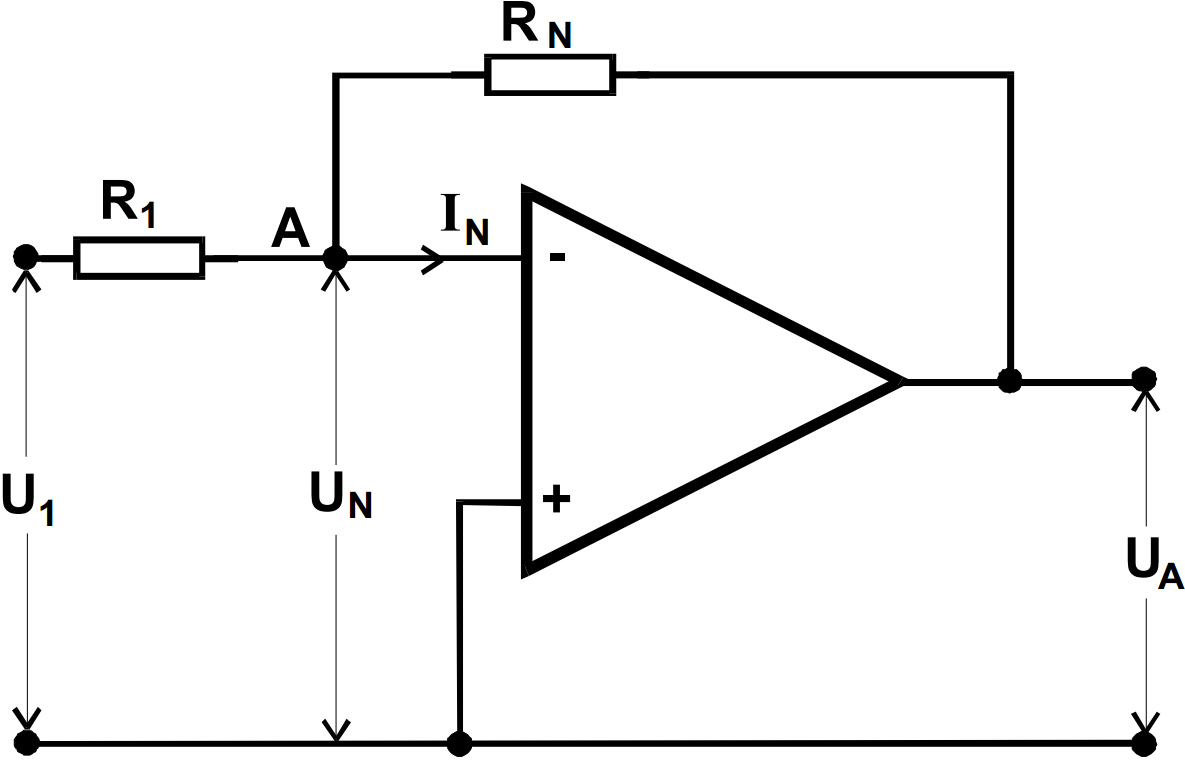
\includegraphics[width=0.5\textwidth]{img/linamp.png}
	\caption{Gegengekoppelter invertierender Linearverstärker \cite{v51}}
	\label{fig:linamp}
\end{figure}

Aufgrund der hohen Leerlaufverstärkung des Operationsverstärkers ist der Spannungsbereich, in dem der OP selbst als Verstärker eingesetzt werden kann, sehr klein.

Eine bessere Verstärkung wird erreicht, wenn der OP in Gegenkopplung betrieben wird.
Dazu wird der Ausgang über einen Widerstand an den invertierenden Eingang angeschlossen.
Das Anschließen an den nicht-invertierenden Eingang wird entsprechend Mitkopplung genannt.
Die Gegenkopplung führt dazu, dass eine positive Spannungsdifferenz der Eingänge zu einer Verringerung von $U_A$, und über die Rückkopplung auch von $U_N$.
Dies führt dazu, dass die Differenz von $U_p$ und $U_N$ verschwindet.
Für rückgekoppelte Operationsverstärker gilt allgemein, dass die beiden Eingänge auf dem gleichen Potenzial liegen.

Beim Linearverstärker, der in Abbildung \ref{fig:linamp} dargestellt ist, liegen folglich beide Eingänge auf Masse.
Es folgt
\begin{align}
	U_1 &= U_{R_1} \quad \text{und} \\
	U_A &= U_{R_N}.
\end{align}

Aufgrund des hohen Eingangswiderstands des OPs wird der Strom $I_N$ vernachlässigt.
Die Ströme durch $R_1$ und $R_N$ sind gleich.
\begin{align}
	I_{R_1} = I_{R_N} \\
	\frac{U_1}{R_1} = \frac{U_A}{R_N} \\
	V' = \frac{U_A}{U_1} = \frac{R_N}{R_1}
\end{align}

Die Verstärkung des gesamten Schaltkreises $V'$ ist somit nur noch von den beiden verwendeten Widerständen abhängig.

Die vorherigen Berechnungen wurden unter Annahme eines idealen OPs gemacht.
Für das reale Bauteil gilt aufgrund der endlichen Leerlaufverstärkung $V$:
\begin{align}
	U_N = -\frac{U_A}{V}
\end{align}
Die beiden Widerstände stellen einen Spannungsteiler dar und es gilt
\begin{align}
	\frac{U_{R_N} - U_1}{U_A - U_1} = \frac{R_1}{R_1 + R_N}.
\end{align}
Daraus ergibt sich für die Gesamtverstärkung
\begin{align}
	\frac{1}{V'} = \frac{U_1}{U_A} = \frac{1}{V} + \frac{R_1}{R_N} \left(1 + \frac{1}{V}\right) \approx \frac{1}{V} + \frac{R_1}{R_N}.
\end{align}

\subsubsection{Umkehr-Integrierer}

\begin{figure}
	\centering
	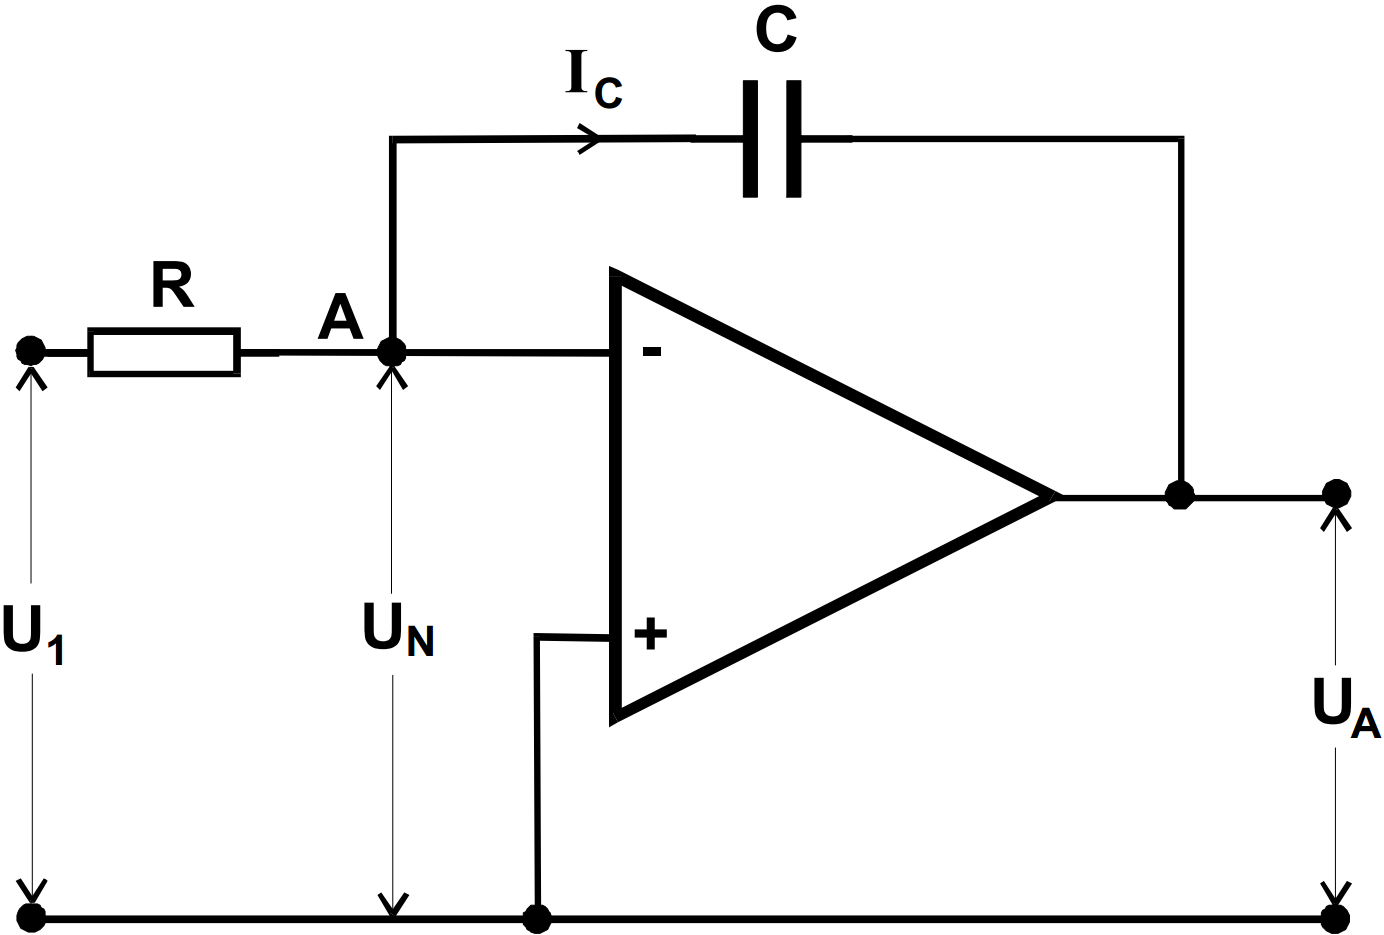
\includegraphics[width=0.5\textwidth]{img/int.png}
	\caption{Umkehr-Integrierer \cite{v51}}
	\label{fig:int}
\end{figure}

\subsubsection{Umkehr-Differenzierer}

\begin{figure}
	\centering
	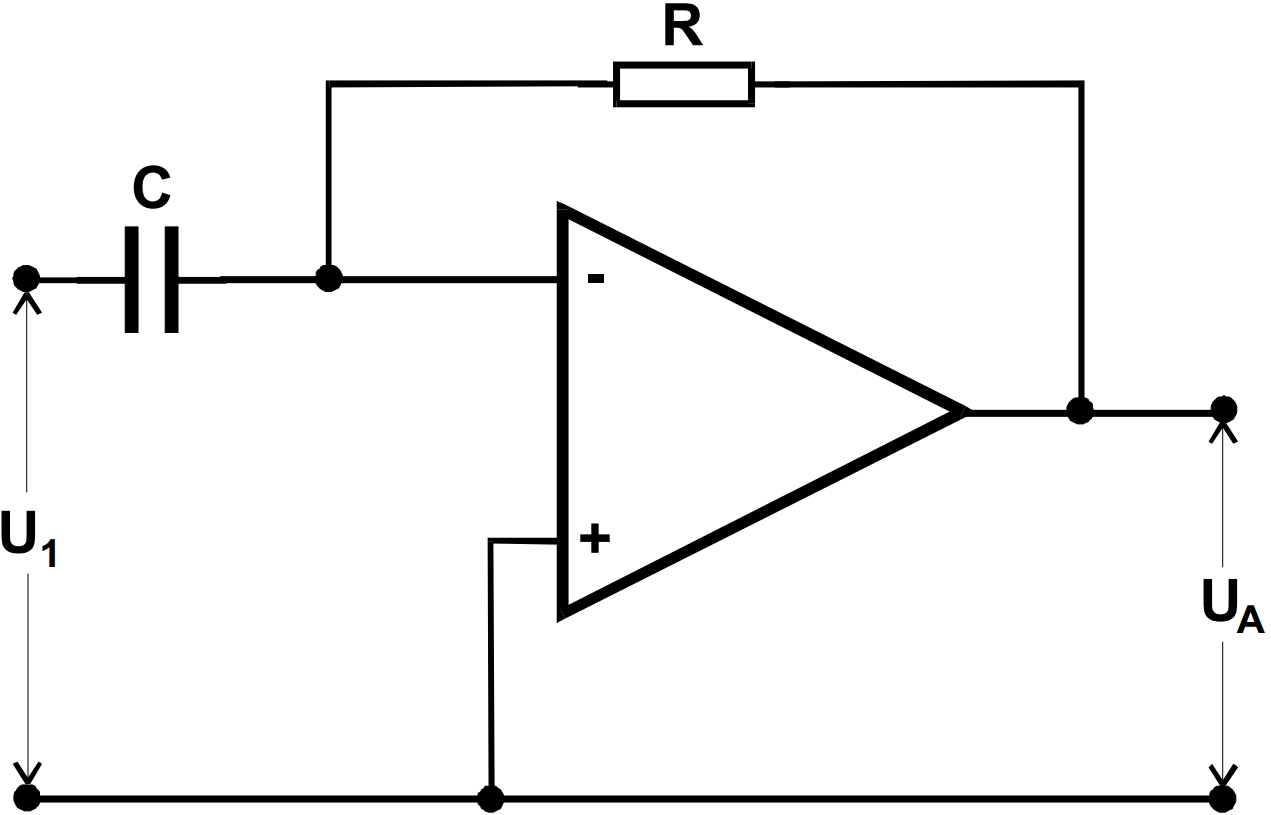
\includegraphics[width=0.5\textwidth]{img/diff.png}
	\caption{Umkehr-Integrierer \cite{v51}}
	\label{fig:diff}
\end{figure}

\subsubsection{Schmitt-Trigger}

\begin{figure}
	\centering
	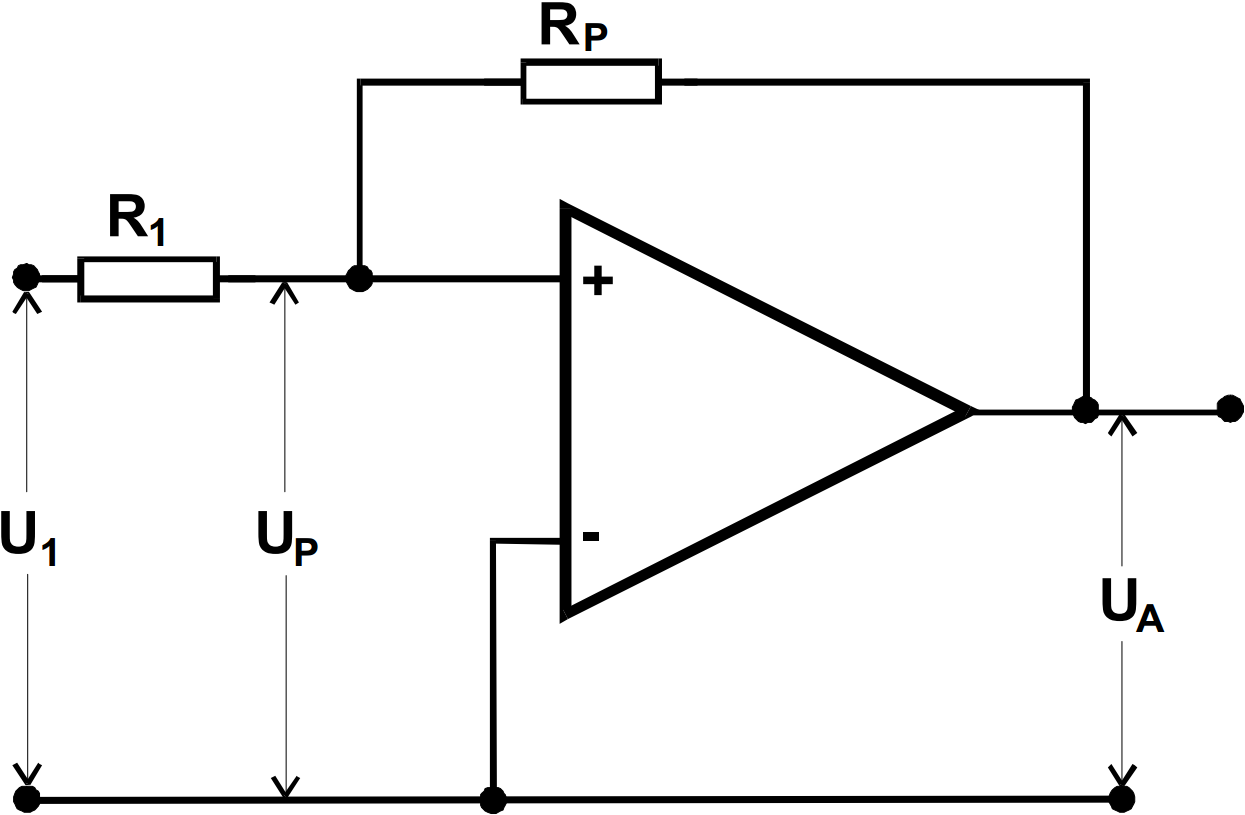
\includegraphics[width=0.5\textwidth]{img/schmitt.png}
	\caption{Schmitt-Trigger \cite{v51}}
	\label{fig:schmitt}
\end{figure}

\subsubsection{Oszillator}

\begin{figure}
	\centering
	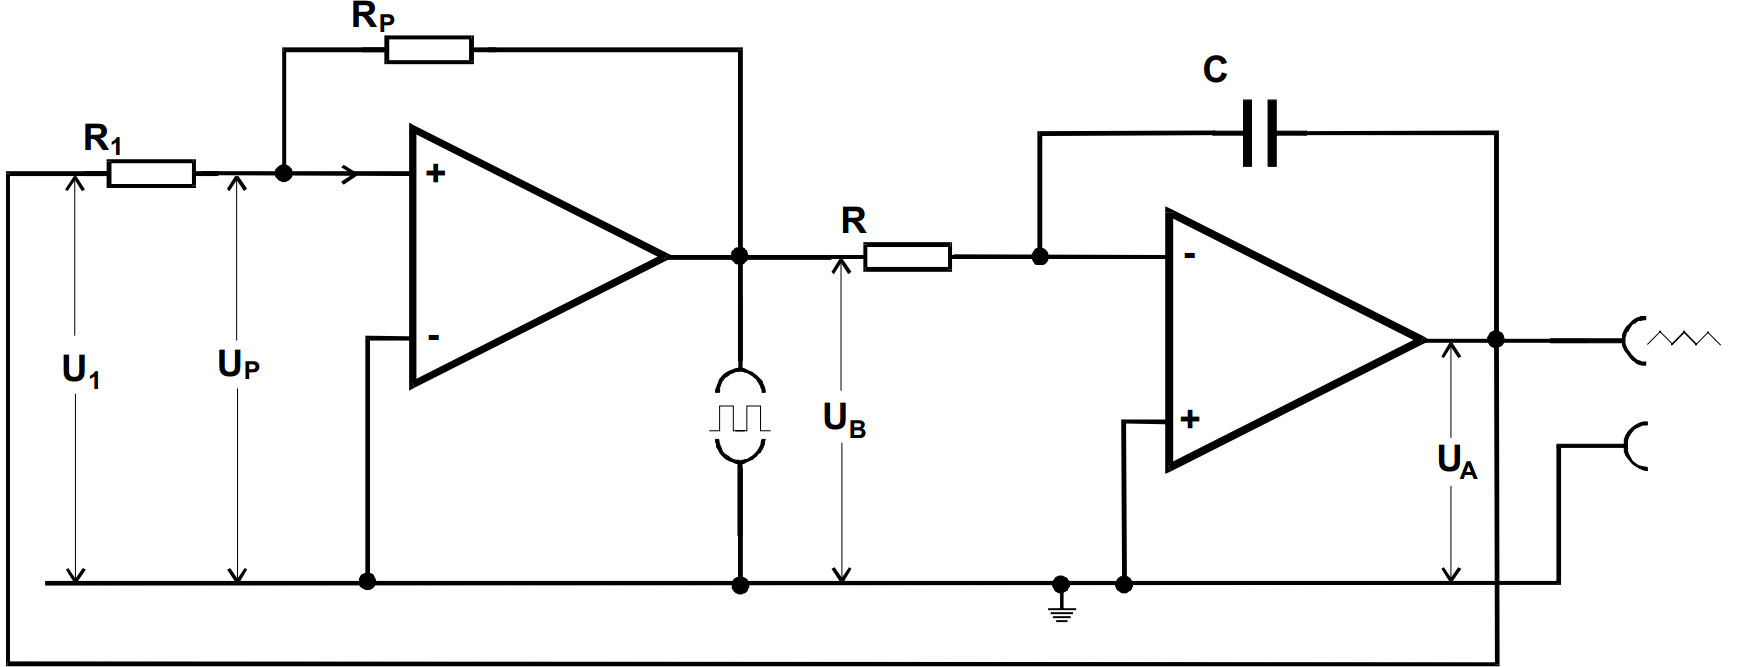
\includegraphics[width=0.5\textwidth]{img/oszi.png}
	\caption{Dreiecks- und Rechteckgenerator \cite{v51}}
	\label{fig:oszi}
\end{figure}

\subsubsection{Sinusgenerator}

\begin{figure}
	\centering
	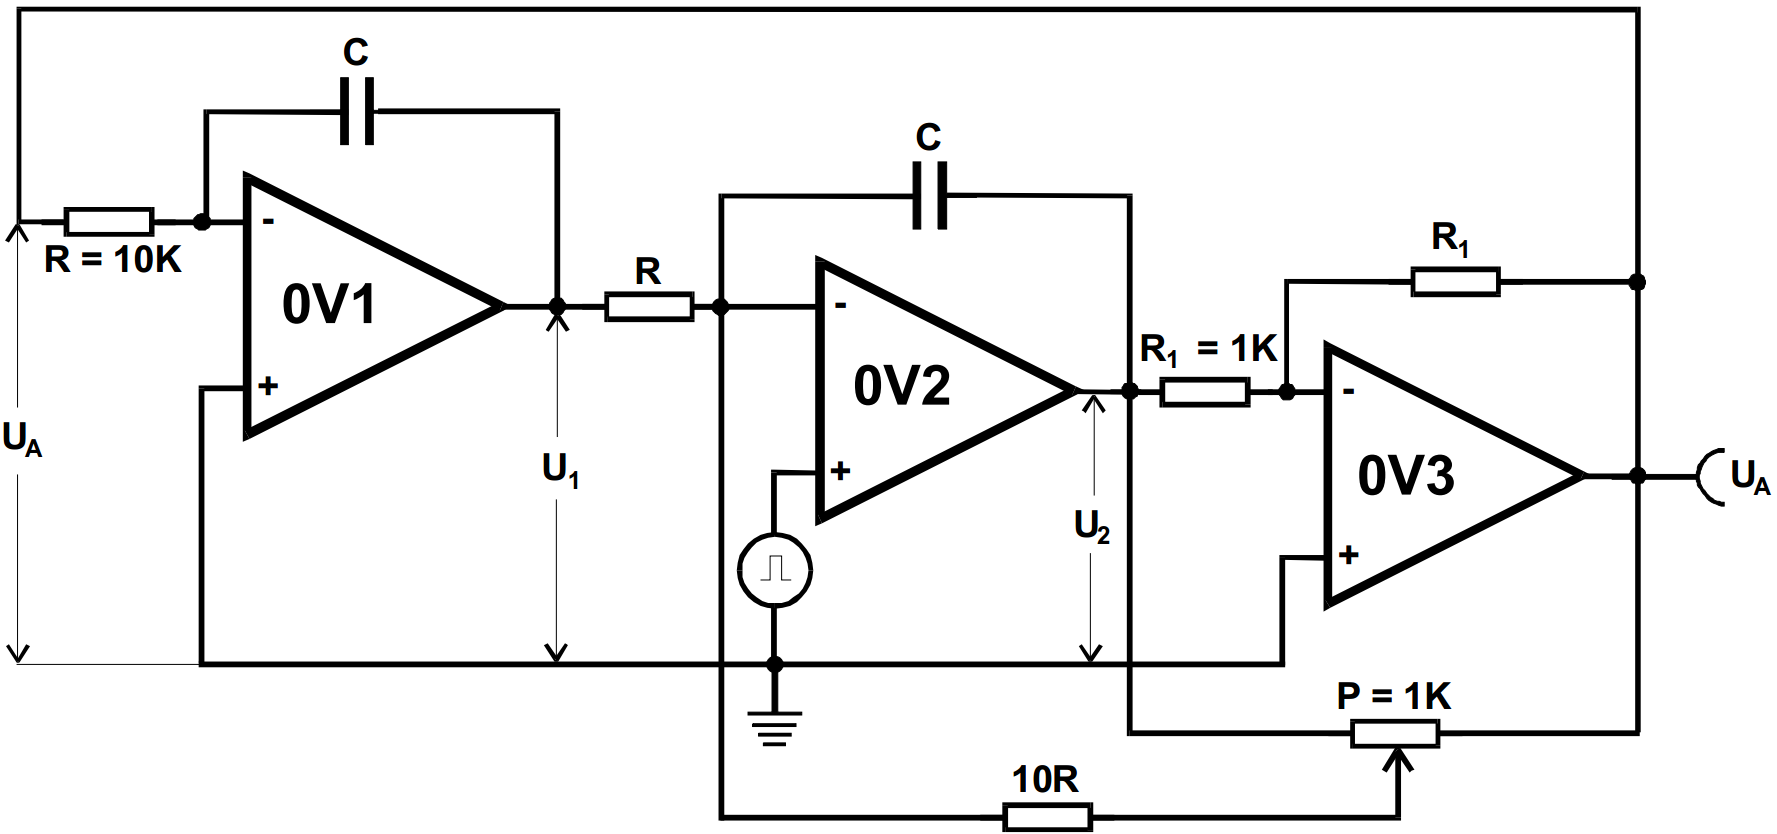
\includegraphics[width=0.5\textwidth]{img/sinus.png}
	\caption{Schaltung für ein gedämpftes Sinussignal \cite{v51}}
	\label{fig:sin}
\end{figure}

\subsubsection{Logarithmierer und Exponenzierer}

\begin{figure}
	\centering
	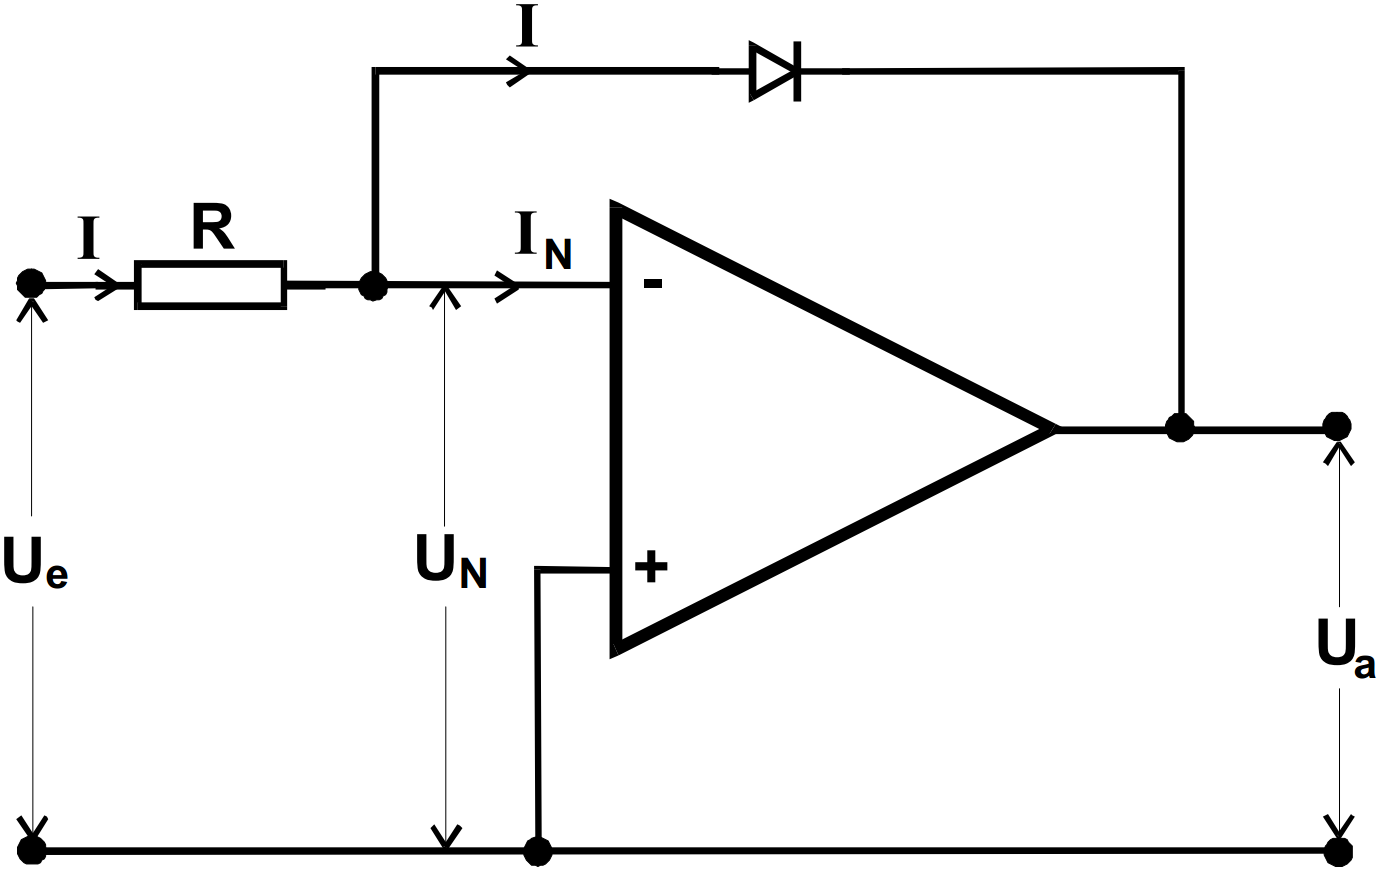
\includegraphics[width=0.5\textwidth]{img/log.png}
	\caption{Logarithmierer \cite{v51}}
	\label{fig:log}
\end{figure}

\begin{figure}
	\centering
	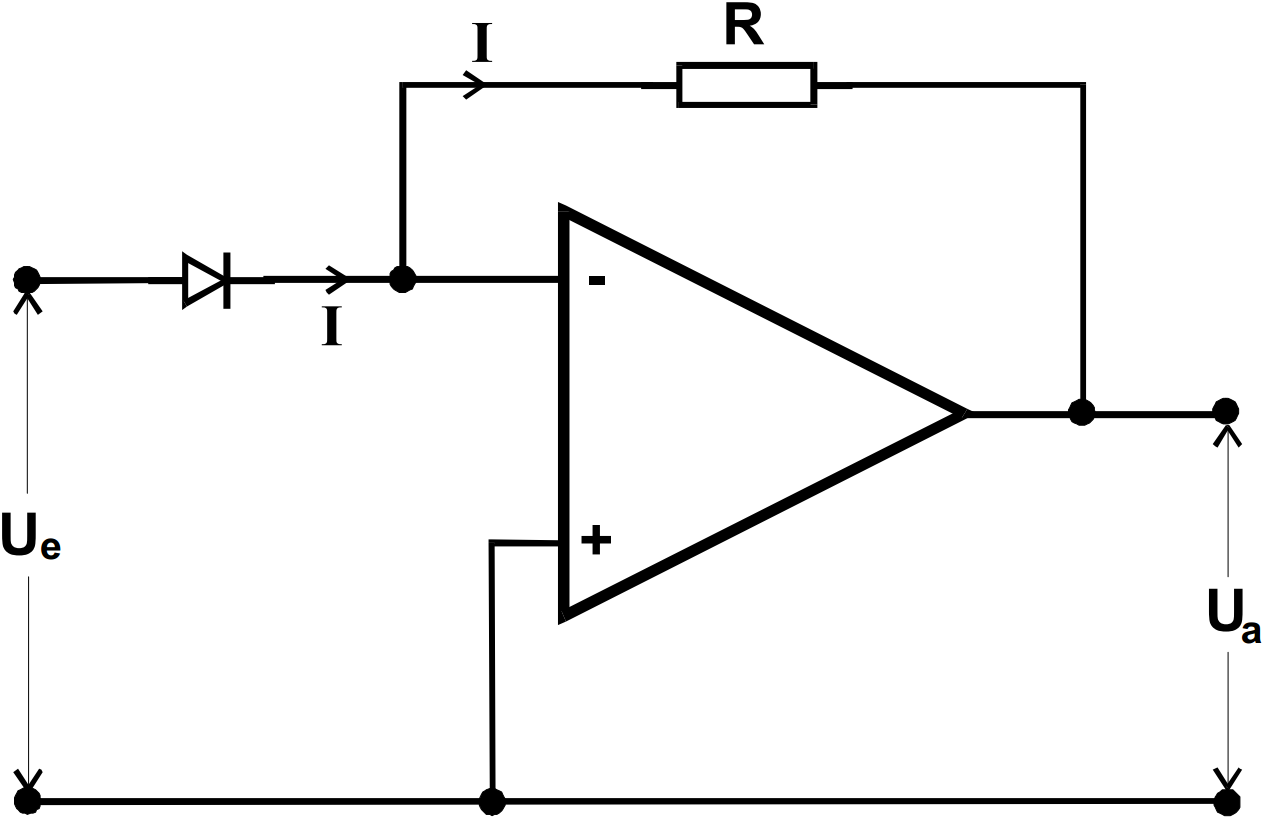
\includegraphics[width=0.5\textwidth]{img/exp.png}
	\caption{Exponenzierer \cite{v51}}
	\label{fig:ep}
\end{figure}
